\chapter{A Molecule's Shape Determines What It Can Do}

\begin{kaichang}
Peel an orange, get a little peel oil on your fingertips, and smell it: that fresh orange scent is familiar to almost everyone. Now peel a lemon and do the same. The scent immediately changes channels---sharp and bright, unmistakably different from orange.

Here is something strange. The main scent molecules in orange and lemon peel oils contain exactly the same numbers of atoms: 10 carbons and 16 hydrogens. Their atoms are even connected in exactly the same order. Both formulas are \chem{C_{10}H_{16}}, and diagrams of ``which atom connects to which'' match perfectly. Yet their smells differ: one suggests orange, the other lemon.

Where is the difference hiding? Make a guess and write it down; we will reveal the answer at the end. Here is your one clue: it is not in the ``parts list,'' but in three-dimensional space.
\end{kaichang}

\section{Smell First: Shape Can Be ``Felt''}

We cannot see individual molecules, but everyday life repeatedly reminds us that molecular \textbf{shape} has consequences.

Water and dry ice make an excellent pair. Both water and carbon dioxide contain oxygen and have exceedingly simple compositions, yet one is liquid at room temperature and the other gas. Dry ice even skips melting, jumping straight from solid to gas amid billowing stage fog. Sugar dissolves in water while sand stays put; evaporating alcohol cools the back of your hand; one pill treats an illness while another with an almost identical molecular formula may do nothing or even cause harm.

Your nose and skin provide more direct evidence. Camphor mothballs release molecules through gaps in plastic bags, scenting a whole wardrobe, whereas an iron nail stored alongside them smells of nothing. Camphor molecules are both volatile and shaped to fit a particular receptor pocket in your nose; iron's atomic crystal holds firmly together with no intention of taking flight. Summer sunscreen is also carefully designed shape engineering: molecular frameworks enable absorption of ultraviolet energy, turning skin-damaging radiation into harmless heat. Right-shaped molecules are absorbed, smelled, and used; wrong-shaped ones slip past your senses and body as though nonexistent.

Neither ``which atoms'' nor, often, ``which connections'' explains these differences. The key lies in a dimension we have not yet examined seriously. A molecule is not a flat drawing but an object in three-dimensional space. Atoms and electron clouds occupy regions, together producing a definite \textbf{geometrical shape}. The rule behind this chapter is surprisingly simple: \textbf{negative charges repel, so electron pairs around a central atom push apart until they are as far from one another as possible}. Most molecular shapes are geometrical consequences of this plain rule.

\section{Why Electron Pairs Push One Another Apart}

Zoom into Chapter 19's covalent molecules. Around a central atom are two kinds of electron cloud: \textbf{bonding pairs}, shared by two atoms (initially count each double or triple bond as one cloud), and \textbf{lone pairs}, belonging only to the central atom and not bonding. Both are negative electron clouds, and negative charges do one thing to each other: repel.

How does repulsion arrange them? Imagine standing in a room's center, surrounded by noisy balloons that dislike one another and each want maximum separation:

\begin{itemize}[itemsep=2pt]
\item 2 balloons: one on each side, making a \textbf{straight line} at $180^{\circ}$.
\item 3 balloons: all in one plane, $120^{\circ}$ apart, making a \textbf{planar triangle}.
\item 4 balloons: a plane accommodates at most 3; the fourth spreads them into three dimensions---the vertices of a regular \textbf{tetrahedron}, about $109.5^{\circ}$ apart.
\end{itemize}

Chemists call this the valence-shell electron-pair repulsion model, VSEPR (pronounced ``vesper''). It follows from Chapter 17's general principle: systems settle into lower-energy states, and separated electron pairs have lower repulsion energy. Molecules have neither eyes nor intentions; electrostatic repulsion ``pushes'' their shape into being.

\begin{shiyan}
\textbf{Balloon Molecular Models (Try at Home)}

Materials: 4--6 identical long balloons and some string or rubber bands.

Procedure: inflate the balloons into long shapes of similar size, without overinflating, and knot each one. Tie 2 balloons tightly together at their middle sections, release them, and observe their natural arrangement. Repeat with bundles of 3 and 4 tied at their midpoints.

What to observe: do 2 balloons naturally form a line? Do 3 flatten into a ``Mercedes badge''? Can 4 lie flat, or do they rise into a three-dimensional ``tripod plus one upright''? Finally, squeeze one balloon in the four-balloon bundle firmly with your hand (representing a lone pair), and see whether the angles between the other three shrink.

Safety note: balloons can burst suddenly; keep knots away from your eyes while tying. Collect fragments promptly to prevent small children or pets from swallowing them.

The model's limits also matter: balloons represent only electron clouds repelling and occupying space. Real molecules contain neither rubber skins nor colors.
\end{shiyan}

\begin{qiaoliang}
Why is the tetrahedral angle $109.5^{\circ}$ rather than $90^{\circ}$ or $120^{\circ}$? Four mutually repelling points on a sphere have only one maximally separated arrangement: a regular tetrahedron's vertices. Simple geometry shows that any two vertices subtend $\arccos(-1/3) \approx 109.5^{\circ}$ at its center.

Now consider two ``squeezed'' numbers. Ammonia, \chem{NH_3}, also has 4 pairs around nitrogen, but 1 is a lone pair. Attracted by only one nucleus, its cloud spreads more ``widely'' and repels more strongly, pressing the 3 bonding pairs down and reducing H--N--H from $109.5^{\circ}$ to about $107^{\circ}$. Water, \chem{H_2O}, has 2 lone pairs and double the squeezing, leaving H--O--H at about $104.5^{\circ}$. No need to memorize these three numbers---$109.5^{\circ}$, $107^{\circ}$, $104.5^{\circ}$. Remember that ``lone pairs are bossier; each extra pair squeezes the angle a little more.''
\end{qiaoliang}

\section{Four Basic Shapes and Their ``Calling Cards''}

Applying VSEPR to Chapter 19's Lewis structures takes three steps: count all electron pairs around the central atom; distinguish bonding and lone pairs; spread them as far apart as possible, then name the molecular shape using \textbf{only the atoms' positions}.

Take water through the full process. Oxygen has 6 outer electrons (Chapter 10's ``floor'' knowledge: second row, Group 16). It shares 2 with two hydrogens to form 2 bonding pairs, leaving 4 electrons as 2 lone pairs. Four pairs total give a tetrahedral electron-pair framework. Now locate the atoms: hydrogen occupies 2 vertices, while ``invisible'' lone pairs occupy 2, leaving a bent visible molecule. Repeat with nitrogen: 5 outer electrons make 3 bonds and 1 lone pair, so ammonia is trigonal pyramidal. Carbon's 4 outer electrons all form bonds, making methane a perfect tetrahedron. Notice: once you can count outer electrons, molecular shapes can almost be \textbf{calculated} rather than memorized.

Some familiar ``calling cards'':

\begin{itemize}[itemsep=2pt]
\item \textbf{Linear}: carbon dioxide, \chem{CO_2}. Central carbon has 2 clouds (two double bonds), $180^{\circ}$ apart.
\item \textbf{Trigonal planar}: boron trifluoride, \chem{BF_3}. Three bonding pairs around boron lie $120^{\circ}$ apart, making the molecule flat.
\item \textbf{Tetrahedral}: methane, \chem{CH_4}. All 4 pairs around carbon are bonding, with hydrogens at the four vertices.
\item \textbf{Trigonal pyramidal}: ammonia, \chem{NH_3}. The electron-pair geometry is tetrahedral, but a lone pair occupies one vertex, leaving nitrogen and three hydrogens looking like a triangular pyramid.
\item \textbf{Bent}: water, \chem{H_2O}. Two of its four pairs are lone pairs, and the two hydrogens lie on the same side of oxygen, making a V.
\end{itemize}

Notice the last detail: lone pairs become ``invisible'' when naming molecular shape. Water is bent, not tetrahedral, because our eyes (and instruments) locate atoms. Yet all the pairs, including lone pairs, determine that shape.

Glance at later pages of the ``card collection,'' just to know they exist: 5 pairs spread into a \textbf{trigonal bipyramid} (three in an equatorial triangle, one above and one below, as in \chem{PCl_5}); 6 form an \textbf{octahedron} (above, below, left, right, front, back, as in \chem{SF_6}). The rule never changes: maximize electron-pair separation around the central atom, then see where the atoms lie.

Putting shapes on paper needs symbols. Chemists use ordinary lines for bonds in the paper's plane, \textbf{solid wedges} for atoms projecting toward you, and \textbf{dashed bonds} for atoms behind the paper. Methane is therefore not a flat cross, which gives a false impression, but carbon joined to two hydrogens in the plane, one forward by a wedge, and one behind by a dashed bond. You will see this notation repeatedly in later chapters.

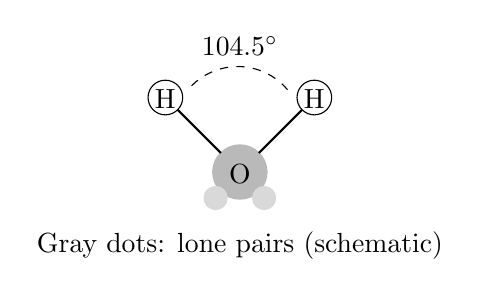
\begin{tikzpicture}[scale=1.1]
\fill[gray!55] (0,0) circle (0.32);
\node at (0,-0.02) {\chem{O}};
\draw[thick] (0.22,0.22) -- (0.72,0.72);
\draw[thick] (-0.22,0.22) -- (-0.72,0.72);
\fill[white] (0.86,0.86) circle (0.2);
\draw (0.86,0.86) circle (0.2);
\node at (0.86,0.84) {\chem{H}};
\fill[white] (-0.86,0.86) circle (0.2);
\draw (-0.86,0.86) circle (0.2);
\node at (-0.86,0.84) {\chem{H}};
\fill[gray!30] (0.28,-0.3) circle (0.14);
\fill[gray!30] (-0.28,-0.3) circle (0.14);
\draw[dashed] (0.55,0.95) arc (40:140:0.75);
\node at (0,1.45) {$104.5^{\circ}$};
\node[align=center] at (0,-0.85) {Gray dots: lone pairs (schematic)};
\end{tikzpicture}

This is a schematic of water's bent shape, a human representation whose circle sizes and shades are not its real appearance. Lone pairs are not two little beads, but two clouds occupying space.

\section{Both Have Polar Bonds, So Why Are Water and Carbon Dioxide Different?}

Now we can fulfill half the title's promise: shape determines properties. The first evidence is water and carbon dioxide, molecules with polar bonds but opposite destinies.

Recall Chapter 19: electronegative oxygen pulls shared electrons toward itself, making both C=O and O--H \textbf{polar bonds}, with one end negative and the other positive. But ``each bond is polar'' and ``the whole molecule is polar'' are different claims, with shape standing between them.

Carbon dioxide is linear: \chem{O=C=O}. Its equal polar bonds point in opposite directions like evenly matched tug-of-war teams. The electron cloud's overall ``center of gravity'' lies exactly in the middle, canceling the positive and negative effects. Thus \chem{CO_2} has \textbf{no overall dipole}. Its molecules barely stick together, naturally making it gaseous at room temperature and allowing solid dry ice to sublime with slight heating.

Water is bent: the two O--H polarities cannot cancel and instead combine to concentrate negative charge at oxygen and expose positive charge at hydrogen. Each molecule is a tiny dipole with negative and positive ends. The consequences are profound: water molecules pull one another, embrace many solute particles, and build ice into an open framework. Chapters 22 and 23 explore these chains of consequences. Here remember their starting point: \textbf{polar bonds + asymmetric shape = polar molecule}.

Now a deceptively shaped example: carbon tetrachloride, \chem{CCl_4}. C--Cl bonds are polar, but four chlorines symmetrically occupy tetrahedral vertices, exactly canceling the four ``tugs.'' With no overall dipole, \chem{CCl_4} does not mix with water but dissolves grease. Shape has ``hidden'' bond polarity.

Apply the same reasoning to two familiar molecules. Ammonia is trigonal pyramidal, its lone pair producing clearly negative and positive ends, so it is polar. This helps explain its ready dissolution in water to make ammonia solution and fertilizer solutions. Methane, \chem{CH_4}, is a perfectly symmetric tetrahedron; all four weak C--H polarities cancel, leaving natural gas almost insoluble in water. Both are ``small molecules,'' yet their solubilities differ enormously. Shape delivers the verdict.

\section{How Shape Was ``Counted''}

How can we know the shape of something invisible? This is one of science's most fascinating questions.

\begin{zhengju}
In 1874, chemists faced a puzzle. Carbon always formed 4 bonds, but how were they arranged in space? Nobody could see them. A young Dutchman, van 't Hoff, and a young Frenchman, Le Bel, who did not know each other, solved it through the same reasoning---not by seeing, but by \textbf{counting}.

Their question was specific. If carbon's 4 bonds lay flat, perhaps toward a square's corners, dichloromethane, \chem{CH_2Cl_2}, should have two versions: chlorines adjacent or opposite. The same parts would assemble into two different objects. Yet repeated preparation, purification, and comparison worldwide found only \textbf{one} \chem{CH_2Cl_2}. Van 't Hoff proposed that only bonds pointing toward \textbf{a tetrahedron's four vertices} made any two positions necessarily equivalent, with no exchange producing a second version---matching observation.

The model also solved a 26-year-old mystery. In 1848, Pasteur used tweezers under a microscope to sort tartrate crystals into two piles. Their shapes were mirror images like left and right gloves; dissolved in water, one rotated polarized light left and the other right. Nobody could explain the molecular reason. Tetrahedral carbon predicted that carbon attached to 4 \textbf{different} groups could give two mirror-image molecules with almost identical chemical properties, differing only in optical rotation and ``matching another hand.'' Tartaric acid was just such a molecule.

There were objections. The established authority Kolbe publicly mocked van 't Hoff for ``chasing phantoms'' and treating imagined spatial structures as science. Stronger evidence delivered the verdict. Early-twentieth-century X-ray crystallography inferred real atomic positions from diffraction patterns. In diamond, carbon's four bonds really met at $109.5^{\circ}$. A shape guessed by ``counting isomers'' had been confirmed by direct measurement. Remember the method: a good structural model rests not on seeing, but on making testable predictions.
\end{zhengju}

\section{When This Model Fails}

VSEPR is a favorite from middle school through university, but it is an \textbf{empirical model} with a definite range.

It is almost unfailingly successful for small main-group molecules with 2--6 pairs around the central atom, but often fails for transition-metal complexes. There, d orbitals (Chapter 9's electron ``apartment layouts'') enter bonding and complicate repulsion. VSEPR tells us pairs ``want to stay apart,'' but not the details of electron-cloud distribution; quantum calculations provide the finer picture. Resonance structures from Chapter 19, such as ozone, \chem{O_3}, also require a Lewis electron-pair count before VSEPR can begin.

Another metaphor needs immediate dismantling. You may have heard of ``hybrid orbitals'': carbon's 1 s and 3 p orbitals ``mix'' into four equivalent $\mathrm{sp^3}$ orbitals pointing tetrahedrally. Remember what they are: a convenient quantum-mechanical \textbf{accounting model}, not objects visible through an electron microscope. Experiments measure a molecule's total electron density and bond angles; nobody has ``photographed'' a hybrid orbital. A useful model need not be a physical object---an essential lesson in scientific thinking.

Finally, molecules are not statues. Bonds act like springs, with atoms continually vibrating around equilibrium positions; single bonds also rotate, changing molecular ``posture.'' Saying water's angle is $104.5^{\circ}$ describes an average picture. For large molecules such as glucose and proteins, overall shape comes from thousands of folds and twists. One atom's VSEPR geometry is only one puzzle piece. Chapter 48 explores proteins as ``folded molecular machines.''

\begin{wuqu}
``Textbooks show oxygen as red balls, hydrogen as white balls, and bonds as sticks---so that is what molecules look like.''

Overly realistic illustrations create this misconception. Atoms have no color (color comes from molecular absorption of visible light; an individual atom's ``color'' is not defined). Bonds are not sticks but electron clouds with higher probability between two nuclei. Molecular edges are not sharp balloon skins; their clouds gradually fade. Ball-and-stick, space-filling, and wedge-and-dash diagrams are \textbf{representations serving different purposes}. Ball-and-stick best shows connections and angles; space-filling comes closest to molecular ``outlines.'' All are maps, not territory. Judge a molecular diagram not by ``how realistic it looks,'' but by whether it clearly answers the question it is meant to explain.
\end{wuqu}

\section{Back to the Orange}

Now for the opening mystery. Orange and lemon peel oils feature the same molecule, limonene, \chem{C_{10}H_{16}}, with identical connections. The difference is \textbf{mirror imagery}.

Hold out both hands, palms up, thumbs outward. Their patterns and finger connections are ``identical,'' yet a left hand cannot be superimposed on a right. This is \textbf{chirality}. Limonene has a carbon attached to 4 different groups, giving two nonsuperimposable mirror-image versions. One mainly smells of orange; the other suggests lemon. Mint and coriander seeds (caraway) likewise differ through a mirror-image pair, carvone.

Why can noses distinguish mirror images? Your smell receptors are proteins, molecular machines with specific three-dimensional ``pockets.'' An odor molecule entering the nose must fit a pocket to trigger a nerve signal. Left- and right-handed molecules fit the same pocket differently, triggering different signal strengths and thus different perceived smells. The causal chain is complete: electron-pair repulsion determines shape, shape determines receptor fit, and fit determines smell. \textbf{Shape is function}, a principle extending to this book's final chapter. Chirality's story is far from finished; Chapter 42 treats it in detail.

Chirality affects more than scent. In the late 1950s, thalidomide was marketed as a sedative. Its molecule also has a ``chiral center'': one mirror image sedates, while the other interferes with fetal development, causing birth defects in more than ten thousand babies in one of pharmaceutical history's most painful lessons. Later research found that the mirror images interconvert in the body, so producing only the ``good'' one cannot eliminate the risk. A direct legacy is that today's drug approvals require studying each mirror image separately. More than half the modern drugs in your medicine cabinet are single-mirror-image, ``one-handed'' molecules.

Industry deliberately exploits shape as function. Fragrance factories no longer squeeze oil from tonnes of orange peel, but directly synthesize particular mirror images of limonene and carvone. With the right shape, the ``orange'' smells like orange. Fertilizer production's Haber process also relies on specific arrangements of catalyst surface atoms to turn nitrogen and hydrogen into ammonia. Nitrogen molecules lie on metallic ``atomic steps,'' where suitably shaped sites hold, weaken, and split them. Chapter 30 explains how catalysts find alternative routes. More familiar is dishwashing liquid: molecules with water-loving and oil-loving ends have just the two-faced elongated shape needed to insert between oil droplets and water, prying grease from plates so it washes away. In the molecular world, no abstract ``effectiveness'' exists: all function is written in shape.

Mirror-image molecules are subtle, but how small are molecules themselves? Estimate the order of magnitude. Water molecules are about $3\times 10^{-10}\,\mathrm{m}$ wide (0.3 nanometers). A drop weighs about 0.05 grams; divide by water's molar mass, $18\,\mathrm{g/mol}$, to get about $2.8\times 10^{-3}\,\mathrm{mol}$. Multiplying by Avogadro's constant, $\ud{6.02\times 10^{23}}{mol^{-1}}$, gives about $1.7\times 10^{21}$ molecules. Lined up, they span about $1.7\times 10^{21} \times 3\times 10^{-10}\,\mathrm{m} \approx 5\times 10^{11}\,\mathrm{m}$, or 500 million kilometers---over three Earth--Sun distances. One drop holds that many ``tiny shaped things,'' each bent molecule casting its vote for ``water is liquid.''

\section{What Remains After Shape?}

Starting from repulsion, this chapter took molecules' ``three-dimensional ID photos'': linear, trigonal planar, tetrahedral, trigonal pyramidal, and bent. Shape explained water's polarity, dry ice's sublimation, citrus scents, and drugs' benefits and disasters.

But one piece is missing. Water is polar---\textbf{then what}? What happens when polar molecules approach? Does a negative end pull a positive one? These very attractions make water liquid and methane gas at room temperature, let geckos walk on ceilings, and shrink dewdrops into balls. Such ``not-quite-bonding, yet real'' intermolecular attractions are the subject of the next chapter, Chapter 22. Water takes them to extremes, producing hydrogen bonds, floating ice, and Earth's climate on Chapter 23's stage. Chapter 42 takes you through chirality's maze: why your amino acids are almost all ``left-handed'' and your sugars almost all ``right-handed.''

\begin{tiaozhan}
\textbf{Hybrid Orbitals: A Successful ``Accounting Method'' (Optional)}

Carbon's electron configuration is $1s^2 2s^2 2p^2$, apparently leaving only 2 unpaired p electrons. How can it form four equivalent bonds? Quantum mechanics describes bonding by recombining the mathematical expressions for one 2s and three 2p orbitals into four completely equivalent ``$\mathrm{sp^3}$ hybrid orbitals,'' automatically pointing toward a regular tetrahedron's vertices. Hybridization calculates through wavefunctions the angle VSEPR guesses through repulsion, letting the models corroborate each other. Similarly, $\mathrm{sp^2}$ hybridization gives a planar triangle (explaining $120^{\circ}$ around double bonds), and sp gives a line (explaining triple bonds).

Remember the boundaries section's warning: experiments measure total electron density, while s, p, and hybrid orbitals are mathematical ways to partition it. Treating hybrid orbitals as real little rooms inside molecules is like treating latitude and longitude as actual strings on Earth's surface. Models are used because their predictions are accurate; use does not turn them into objects.
\end{tiaozhan}

\section*{Try It}

\begin{sikaoti}
\item Both ammonia, \chem{NH_3}, and water, \chem{H_2O}, have four pairs around the central atom. Draw their electron-pair arrangements using different marks for bonding and lone pairs, and explain why ammonia is pyramidal and water bent. Note beside the diagrams that these are representations, not little electron beads.
\item Boron trifluoride, \chem{BF_3}, and ammonia, \chem{NH_3}, each have four atoms. Why is one trigonal planar and the other pyramidal? Answer using total and lone-pair counts around the central atom.
\item Carbon tetrachloride's C--Cl bonds are polar, but \chem{CCl_4} as a whole is not. Replace one chlorine with hydrogen to make \chem{CHCl_3}, and a dipole appears. Explain this transformation through tetrahedral geometry.
\item Sulfur dioxide, \chem{SO_2}, has three clouds around sulfur, including one lone pair. Predict its shape and polarity, explaining your reasoning. Atmospheric \chem{SO_2} dissolves in water to form acid rain. Does your prediction agree?
\item Your body can use only ``left-handed'' amino acids to build proteins. Draw an information flowchart from ``mirror-image molecular shape'' through ``receptor or enzyme's three-dimensional pocket'' to ``whether the body can use it.'' Use the same chart to explain why orange- and lemon-scented limonene have identical formulas.
\end{sikaoti}
